\documentclass{article}

\usepackage{amsmath, amsthm, amssymb, amsfonts}
\usepackage{thmtools}
\usepackage{graphicx}
\usepackage{setspace}
\usepackage{geometry}
\usepackage{float}
\usepackage{hyperref}
\usepackage[utf8]{inputenc}
\usepackage[english]{babel}
\usepackage{framed}
\usepackage[dvipsnames]{xcolor}
\usepackage{tcolorbox}

\usepackage{derivative}
\usepackage{siunitx}

\hypersetup{
    colorlinks=true,
    linkcolor=black,
    citecolor=blue,
    urlcolor=cyan
}

\graphicspath{{images/}}

\colorlet{LightGray}{White!90!Periwinkle}
\colorlet{LightOrange}{Orange!15}
\colorlet{LightGreen}{Green!15}
\colorlet{LightBlue}{Cyan!30}
\colorlet{LightRed}{Red!30}

\newcommand{\HRule}[1]{\rule{\linewidth}{#1}}

\declaretheoremstyle[
    name=Theorem,
    headpunct=\newline % Forces a newline after theorem title
]{thmsty}
\declaretheorem[style=thmsty,numberwithin=section]{theorem}
\tcolorboxenvironment{theorem}{colback=LightGray}

\declaretheoremstyle[
    name=Proposition,
    headpunct=\newline
]{prosty}
\declaretheorem[style=prosty,numberlike=theorem]{proposition}
\tcolorboxenvironment{proposition}{colback=LightOrange}

\declaretheoremstyle[
    name=Principle,
    headpunct=\newline
]{prcpsty}
\declaretheorem[style=prcpsty,numberlike=theorem]{principle}
\tcolorboxenvironment{principle}{colback=LightGreen}

\declaretheoremstyle[
    name=Example,
    headpunct=\newline
]{exsty}
\declaretheorem[style=exsty,numberlike=theorem]{example}
\tcolorboxenvironment{example}{colback=LightBlue}

\declaretheoremstyle[
    name=Answer,
    headpunct=\newline
]{anssty}
\declaretheorem[style=anssty]{answer}
\tcolorboxenvironment{answer}{colback=Goldenrod}

\declaretheoremstyle[
    name=Definition,
    headpunct=\newline
]{defsty}
\declaretheorem[style=defsty,numberlike=theorem]{definition}
\tcolorboxenvironment{definition}{colback=LightRed}


\setstretch{1.2}
\geometry{
    textheight=9in,
    textwidth=5.5in,
    top=1in,
    headheight=12pt,
    headsep=25pt,
    footskip=30pt
}

% ------------------------------------------------------------------------------

\begin{document}

% ------------------------------------------------------------------------------
% Cover Page and ToC
% ------------------------------------------------------------------------------

\title{ \normalsize \textsc{}
		\\ [2.0cm]
		\HRule{1.5pt} \\
		\LARGE \textbf{\uppercase{AP Physics C}
		\HRule{2.0pt} \\ [0.6cm] \LARGE{yeah} \vspace*{10\baselineskip}}
		}
\date{}
\author{\textbf{Franklin Chen} \\ 
		22 March 2026 - 13 May 2026}

\maketitle
\newpage

\tableofcontents
\newpage

% ------------------------------------------------------------------------------

\subsection{Foreword for anybody else using this}
As of writing this, I've already taken AP Physics 1 and 2 and Calc BC, so I'll skim over those stuff.
I steal the images from google. If this violates copyright somehow, please email me and I'll remove it.

\newpage

\section{Unit 1: Kinematics}
\subsection{Scalars and Vectors}
Scalars are numbers. Vectors are vectors. Represent as $\vec{a} = \hat{\imath} + \hat{\jmath} + \hat{k}$.

Dot product of two vectors is the length of one of the vectors projected onto the other multiplied by the length of said other vector. Theta = min angle between two vectors.

\[\vec{a} \cdot \vec{b} = |\vec{a}| |\vec{b}| \cos{\theta}\]

\subsubsection{Cross Product}
Operation that can be applied to two \textbf{three-dimensional} vectors to generate a third vector perpendicular to both vectors.
Use the \textbf{right hand rule} to deterimine which direction the third vector will go.

\begin{principle}[Right Hand Rule]
    To find the geometrical direction of $\vec{a} \times \vec{b}$, hold your right hand out and point your \textit{index} finger in the direction of $\vec{a}$, and your \textit{middle} in the direction of $\vec{b}$.
    Your thumb will point in the direction of $\vec{a} \times \vec{b}$.
        
    \begin{center}
        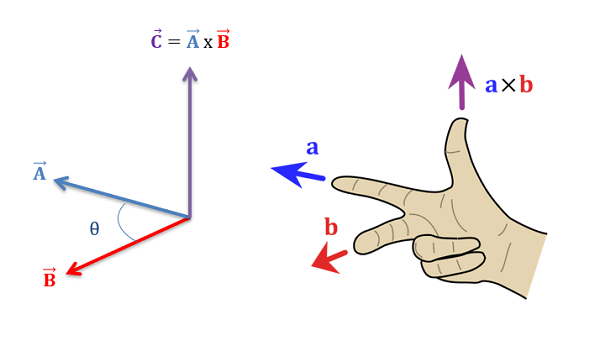
\includegraphics[scale=1.0]{righthand.png}
    \end{center}
\end{principle}

\begin{principle}[Calculating the Cross Product]
    To calculate the cross product between $\vec{A}$ and $\vec{B}$:
    \begin{center}
        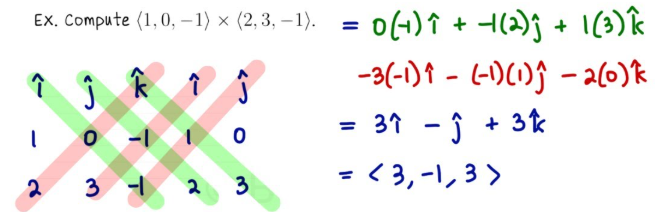
\includegraphics[scale=0.5]{cross.png}
    \end{center}
\end{principle}

Note the following:
\begin{enumerate}
    \item $|\vec{a} \times \vec{b}| = |\vec{a}||\vec{b}|\sin{\theta}$ where theta is the minimum angle betwen the two vectors. Also equal to the area of the parallelogram formed by $\vec{a}$ and $\vec{b}$.
    \item $\vec{a} \times \vec{b} = -(\vec{b} \times \vec{a})$. This property is known as the \textbf{anti-commutativity of the cross product}.
    \item $\vec{a} \times \vec{a} = \vec{0}$ ($\theta = 0$)
\end{enumerate}

\subsection{Displacement, Velocity, and Acceleration}
\[
\vec{v} = \odv{\vec{s}}{t}, a = \odv{\vec{v}}{t} = \odv[2]{\vec{s}}{t} \implies \Delta \vec{s} = \int \vec{v}(t)dt, \Delta \vec{v} = \int \vec{a}(t)dt
\]

Derivatives and intergrals of vector-valued functions can be done component wise.
\[
\vec{s} = x(t)\hat{\imath} + y(t)\hat{\jmath} + z(t)\hat{k} \implies \odv{\vec{s}}{t} = x'(t)\hat{\imath} + y'(t)\hat{\jmath} + z'(t)\hat{k}
\]
\[
\vec{s} = x(t)\hat{\imath} + y(t)\hat{\jmath} + z(t)\hat{k} \implies \int_{t_i}^{t_f}\vec{s}dt = \int_{t_i}^{t_f}x(t)dt + \int_{t_i}^{t_f}y(t)dt + \int_{t_i}^{t_f}z(t)dt
\]

For constant one-dimensional acceleration, kinematic equations apply:
\[\Delta v = \int adt \implies v_f = v_i + at\]
\[\Delta s = \int v(t)dt = \int (v_i + at)dt \implies \Delta s = v_it + \frac{1}{2}at^2\]
\[v_f = v_i + at \implies v_f^2 = v_i^2 + 2v_iat + a^2t^2 \implies v_f^2 = v_i^2 + a(2v_it + at^2) \implies v_f^2 = v_i^2 + 2a\Delta x\]

Falling object experience constant acceleration: $a = g \approx 9.81\unit{\metre \per \second \squared} \approx 10\unit{\metre \per \second \squared}$.
Projectiles experience constant vertical accleration of gravity, but no horizontal acceleration.

\subsection{Representing Motion}
Distance, velocity, and acceleration vs. time graphs exist. Yipee!

\subsection{Reference Frames and Relative Motion}
Let $\vec{v}_{AB}$ = velocity of $A$ relative to $B$.
\[\vec{v}_{AB} = -\vec{v}_{BA}\]
\[\vec{v}_{AC} = \vec{v}_{AB} + \vec{v}_{BC}\]

These are also known as \textbf{Galilean Transformations.} Note these equations will break down near the speed of light due to relativity shit.

\begin{example}
    The president's airplane flies at $250 \unit{\metre \per \second}$ to the east with respect to the air.
    The air is moving at $35 \unit{\metre \per \second}$ to the north with respect to the ground.
    Find the velocity of the president's airplane with respect to the ground.
\end{example}
\begin{answer}
    Let $\hat{\imath}$ = north and $\hat{\jmath}$ = east.
    \[\vec{v}_{PG} = \vec{v}_{PA} + \vec{v}_{AG} = (250\hat{\jmath} + 35 \hat{\imath})\]
    \[|\vec{v}_{PG}| = \sqrt{250^2 + 35^2} \approx 252.4\unit{\metre \per \second}\]
    \[\theta_{PG} = \arctan{\frac{35}{250}} \approx 7.97\unit{\degree} \textrm{ relative to East}\]
\end{answer}


\section{Unit 2: Force and Translational Dynamics}

\section{Unit 3: Work and Power}

\section{Unit 4: Linear Momentum}

\section{Unit 5: Torque and Rotational Dyanmics}

\section{Unit 6: Energy and Momentum of Rotating Systems}

\section{Unit 7: Oscillations}

\section{Unit 8: Electric Charges, Fields, and Gauss's Law}

\section{Unit 9: Electric Potential}

\section{Unit 10: Conductors and Capacitors}

\section{Unit 11: Electric Circuits}

\section{Unit 12: Magnetic Fields and Electromagnetism}

\section{Unit 13: Electromagnetic Induction}
\end{document}